\section{Architecture du projet}

\subsection{Un système client/serveur}

Au premier semestre de cette année, notre étude bibliographique nous à permis d'étudier les deux systèmes de fenêtrages majeurs sous linux, X Window System (implémentation X.org) et le tout jeune Wayland. Cette étude nous a permis de décider de calquer notre futur système de fenêtrage (pron) sur X Window System qui était selon nous, le plus simple et le plus adapté. De plus, l'implémentation X.org étant un projet mûr, il est très bien documenté et les solutions conceptuelles qu'il a utilisé sont validée et fonctionnent.

Notre Système de fenêtrage, sera divisé en deux grandes parties, le serveur graphique en tant que tel, pron et la librairie client implémentant le protocole de communication pron, la pronlib.

Après avoir étudié les solutions existantes pour ce qui est de la gestion des fenêtres, nous avons opté pour un système identique à métacity. Le gestionnaire de fenêtres, guacamole, sera un client à part entière du serveur graphique (pron), qui se contentera d'intercepter certains évènements comme on le verra plus tard.

Enfin, la librairie de widget, sombrero, s'inspirera à la fois de QT (en version 4), et de GTKMM (wrapper pour GTK).

\subsection{Illustration}
  
\begin{figure}[H]
  \centering
  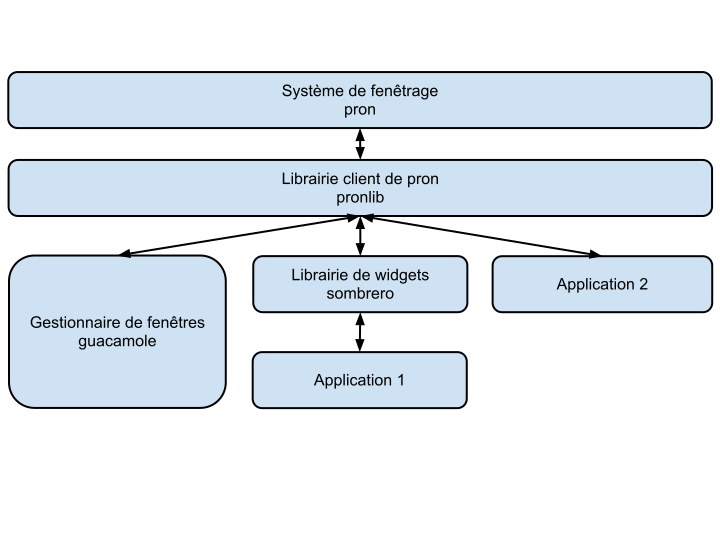
\includegraphics[width=18cm]{images/architecture.png}
  \caption{Architecture}
  \label{fig:architecture}
\end{figure}

\subsection{Langage de programmation}

Après avoir longuement réfléchi, nous somme convaincus qu'une conception objet pour ce projet est appropriée. Il en découle que la famille de languages à utiliser sera les langages objets, notamment le c++. C'est pour cela que TacOS-GUI est écrit c++.


